\section{Extended Attack-Resilience Results}
\label{app:attacks}

Section~\ref{subsec:rq1} reports the malicious-proposer scenario
as the main body's representative attack. Table~\ref{tab:attack-full}
reports the full ten-scenario live attack suite for completeness; all
scenarios were run on the real 7-validator testbed (four validators for the
eclipse/Sybil rows, carried over from an earlier cluster size, not yet
re-run at 7-node scale).

\begin{table}[h]
\caption{Full Attack-Resilience Suite (live)}
\label{tab:attack-full}
\centering
\footnotesize
\begin{tabular}{@{}p{0.04\linewidth}p{0.24\linewidth}p{0.08\linewidth}p{0.08\linewidth}p{0.42\linewidth}@{}}
\toprule
\textbf{\#} & \textbf{Attack} & \textbf{Safety} & \textbf{Diverg.} & \textbf{Attack-specific signal} \\
\midrule
A1 & Eclipse & True & 0 & Filter holds 8/8, nil-prevote ratio 0.0 throughout \\
A2 & Simulated multi-subnet Sybil & True & 0 & Filter holds 8/8 despite 12 attackers \\
A3 & Data withholding & True & 0 & --- \\
A4 & Forged Bitcoin receipt & True & 0 & --- \\
A5 & Withdrawal during \textsc{Sovereign} & True & 0 & Withdrawal correctly blocked; transaction never commits \\
A6 & Malicious proposer & True & 0 & Reported as the main-body representative (Section~\ref{sec:evaluation}) \\
A7 & Censorship & True & 0 & Censoring confirmed real (target tx omitted 9/9 proposer turns); honest reject signals stayed at 0 since the next honest proposer included the tx before the ignore-round threshold fired \\
A8 & Combined (A6 + A1) & True & 0 & Safety held under simultaneous overlap \\
A9 & Double-signing & True & 0 & 6/6 honest validators detected real duplicate-vote evidence; 1-block detection latency \\
A10 & Timeout flood & True & 0 & Cadence held (0.770$\to$0.706 blocks/s); rate limiter dropped 0/0/0/0/0/0 at moderate (20 msg/s) intensity \\
\bottomrule
\end{tabular}
\end{table}

A3 and A4 report no attack-specific signal beyond \texttt{safety\_held}
and \texttt{divergence\_events} because these two attacks (unlike, e.g.,
A5's \texttt{blocked\_correctly} or A9's evidence-detection latency) were
not instrumented with a distinguishing metric in this experiment suite;
the ``---'' reflects that measurement gap honestly rather than implying
a distinguishing signal exists but is omitted.

At 25$\times$ its design threshold (500 msg/s vs.\ a 20 msg/s per-peer cap),
the A10 timeout-flood attack still held cadence (0.825$\to$0.789 blocks/s)
while the rate limiter rejected the large majority of flood traffic
(28{,}071 of $\sim$30{,}000 attempted messages on one validator); validator
CPU usage roughly tripled (2.4--3.3\%$\to$7.85--9.51\%, peak 22.40\%) but
stayed well short of saturation, and memory usage stayed flat. No attack in
Table~\ref{tab:attack-full} drove block production toward zero, and resource
usage under the P2P swarm attacks (A1/A2) stayed modest (under 36\% CPU,
under 147\,MiB memory per validator).

\FloatBarrier
\section{Backend Trade-off: Noir+Honk vs.\ Plonky3}
\label{app:backend}

Section~\ref{subsec:reanchoring} deploys a Noir circuit proved with
Barretenberg's UltraHonk backend for the re-anchoring recovery proof. This
appendix reports a secondary evaluation of an alternative STARK-based
backend, Plonky3, deferred from the main body because no fair, apples-to-apples
comparison currently exists: the deployed circuit's dominant cost is
condition~(e), boundary-signature verification, which accounts for roughly
180$\times$ the circuit's constraint count (6{,}143 opcodes without it vs.\
1{,}097{,}274 with it), and no available Plonky3 configuration implements
this condition.

\begin{table}[h]
\caption{Deployed Circuit: Constant-Cost Scaling (Noir+Honk, Poseidon2)}
\label{tab:reanchor-scaling}
\centering
\footnotesize
\begin{tabular}{@{}rrrr@{}}
\toprule
\textbf{Interval count} & \textbf{Prove time} & \textbf{Verify time} & \textbf{Proof size} \\
\midrule
1   & 38.3 s & 25 ms & 14{,}656 B \\
16  & 41.4 s & 23 ms & 14{,}656 B \\
256 ($N_{\max}$) & 40.4 s & 24 ms & 14{,}656 B \\
\bottomrule
\end{tabular}
\end{table}

Table~\ref{tab:reanchor-scaling} confirms the deployed circuit's
constant-cost, dynamic-padding design (Section~\ref{subsec:reanchoring}):
prove time, verify time, and proof size are all independent of the number
of aggregated \textsc{Sovereign}-interval headers, up to the compiled
maximum of $N_{\max}{=}256$.

\begin{table}[h]
\caption{Backend Comparison, Statement Coverage}
\label{tab:backend-coverage}
\centering
\footnotesize
\begin{tabular}{@{}lccccc@{}}
\toprule
\textbf{Config.} & (a) & (b) & (c) & (d) & (e) \\
\midrule
Noir+Honk (deployed) & \checkmark & \checkmark & \checkmark & \checkmark & \checkmark \\
Plonky3, primitive-only & -- & -- & -- & -- & -- \\
Plonky3, fuller statement & \checkmark & \checkmark & \checkmark & \checkmark & -- \\
\bottomrule
\end{tabular}
\\[2pt]
\footnotesize (a) chain continuity, (b) FSM/withdrawal-lock policy legality,
(c) circuit-breaker adherence, (d) state-root binding, (e) boundary
ed25519-signature verification.
\end{table}

Table~\ref{tab:backend-coverage} makes the coverage gap explicit. Under a
primitive-only comparison (256 chained Poseidon2 permutations, no FSM or
signature logic, i.e.\ neither configuration implements condition~(e)),
Plonky3 produces a substantially larger proof (1{,}278{,}939~B vs.\
14{,}656~B, $\sim$87$\times$) but proves faster (0.044~s vs.\ 0.684~s,
$\sim$15.5$\times$) with a transparent, post-quantum-secure setup versus the
Noir/Honk backend's trusted KZG setup. Under a fuller-statement comparison
that adds FSM legality and root binding (but still omits condition~(e)),
Plonky3 proves in 0.024--0.096\,s with proof sizes of 84--124\,KB across
2--256 headers. \textbf{Neither comparison supports a general ``Plonky3 is
$N\times$ faster'' claim}: both omit the single component that dominates the
deployed circuit's real cost, and implementing boundary-signature
verification in Plonky3 is estimated at 4--7 weeks of dedicated engineering
work, not attempted in this evaluation. We therefore report these numbers
as a scoped, secondary data point on primitive-level backend trade-offs,
not as a claim about the deployed system's alternative-backend performance.

\FloatBarrier
\section{Bitcoin Reorg Depth Reaction}
\label{app:reorg}

Section~\ref{subsec:formal-invariants} states a threat-model boundary --
safety is modeled given Bitcoin reorganizations no deeper than a
configurable finality depth $K_{\text{DEEP\_FINALITY}}$ -- as a condition on
the formal result, not merely a caveat. This appendix reports a live test of
what the running implementation actually does at and beyond that boundary,
using real, forced Bitcoin reorganizations (verified independently against
the resulting block hashes, not assumed from height alone) at five depths in
one 7-node run: \{1, 2, 3, 5, 15\}, with $K_{\text{DEEP\_FINALITY}}{=}2$ and
a suspicious-state threshold of 4.

\begin{figure}[h]
\centering
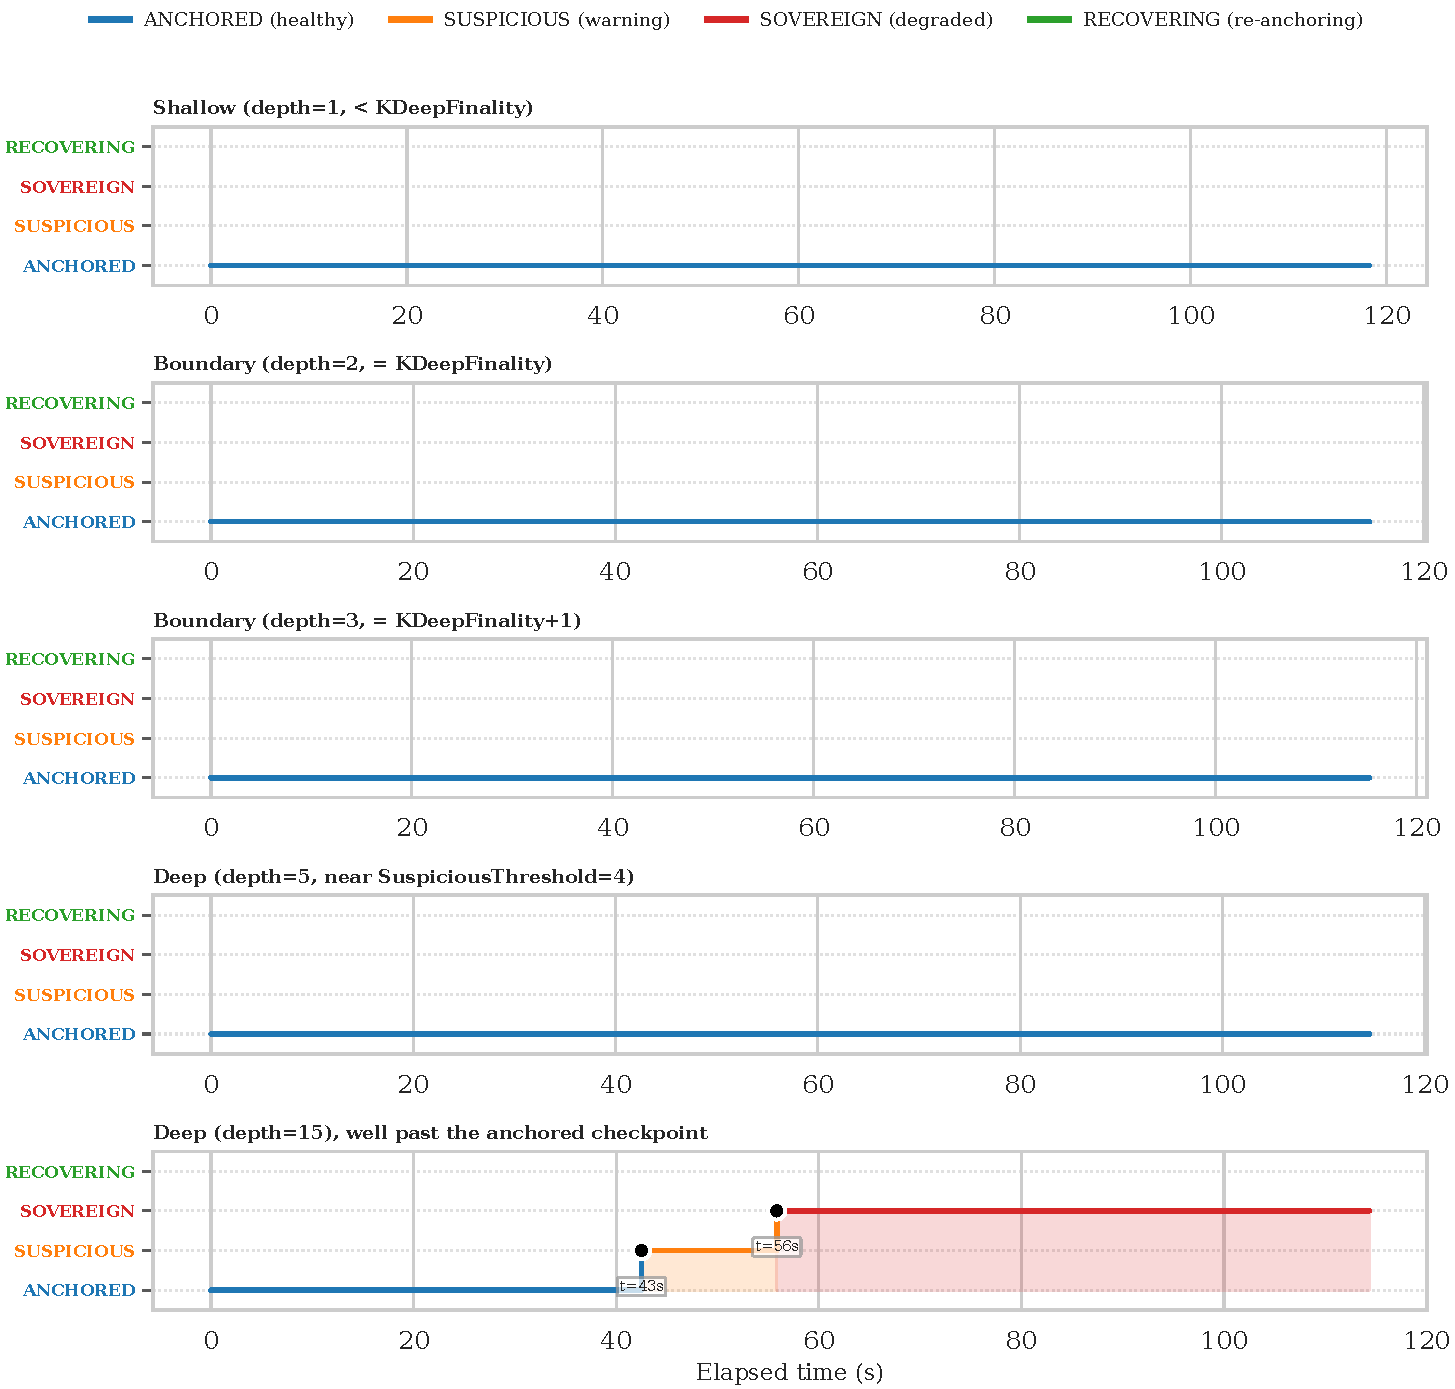
\includegraphics[trim=0 0 0 25pt, clip, width=\linewidth]{figures/figure8_reorg_depth_reaction_live.pdf}
\caption{FSM reaction to real Bitcoin reorgs by depth, 5 trials, live
7-validator testbed. All 7 validators agree at every one of 181 polled
rounds per trial (1{,}267 samples total, 0 RPC errors).}
\label{fig:reorg}
\end{figure}

\FloatBarrier

Table~\ref{tab:reorg} summarizes the result. Depths 1--5 all orphan real,
independently-confirmed blocks, yet none of them trip the FSM: all 7
validators stay \textsc{Anchored} throughout. This is wider tolerance than
the specification's own boundary alone would predict -- the specification
(Section~\ref{subsec:formal-invariants}) only commits to safety \emph{up to}
$K_{\text{DEEP\_FINALITY}}$, leaving deeper reorgs formally out of scope,
yet the anchor-verification routine's no-cache,
re-derive-on-every-call design catches depths~3 and~5 as well, purely as an
implementation-level defense-in-depth property the TLA+ model does not
itself claim. Only at depth~15 -- well past the anchored checkpoint -- does
the FSM react, and it does so correctly and in lockstep: all 7 validators
transition \textsc{Anchored}$\to$\textsc{Suspicious} at $t{=}43$\,s and
$\to$\textsc{Sovereign} at $t{=}56$\,s.

\begin{table}[h]
\caption{FSM Reaction to Real Bitcoin Reorgs by Depth}
\label{tab:reorg}
\centering
\scriptsize
\begin{tabular}{@{}p{0.16\linewidth}p{0.24\linewidth}p{0.44\linewidth}@{}}
\toprule
\textbf{Depth} & \textbf{Reorg confirmed?} & \textbf{FSM reaction} \\
\midrule
1 (below $K_{\text{DEEP}}$) & N/A (too shallow) & Stays \textsc{Anchored} \\
2 ($=K_{\text{DEEP}}$)      & Yes & Stays \textsc{Anchored} \\
3 ($=K_{\text{DEEP}}{+}1$)  & Yes & Stays \textsc{Anchored} \\
5 (near threshold${=}4$)    & Yes & Stays \textsc{Anchored} \\
15 (past checkpoint)        & Yes & \textsc{Suspicious}~(43s) $\to$ \textsc{Sovereign}~(56s) \\
\bottomrule
\end{tabular}
\end{table}

We report this honestly as an uncharacterized gap rather than a fully
mapped boundary: the exact crossover between depth~5 (no reaction) and
depth~15 (reaction) was not swept at finer granularity in this run.
Sensor-level detection (the Bitcoin SPV check firing on a
re-verified reorg) and FSM-level reaction (a committed state transition) are
two different layers with two different tolerances -- the former fires at
every tested depth $\geq 2$, the latter only once the resulting
Bitcoin finality gap exceeds the suspicious-state threshold -- and this run
measures that gap up to depth~5 rather than merely assuming it from the
specification.